\chapter{Bilan et perspectives}
\label{chap:bilan}

\section{Organisation du travail}
\label{sec:orga}
  \subsection{Application du référentiel qualité interne}
  
  Nous exposons ici les éléments fourni par SII ayant guidé de manière significative la conduite du projet. 
  Ceux-ci seront plus ou moins détaillés notamment au temps ayant été consacré à leur mise en place.
  
  Les premiers éléments oraganisationnels qui ont été formalisés s'incarnent par deux documents de spécification appelés \gls{STBL} et \gls{DCL}.
  Le premier vise, comme son nom l'indique, à exprimer le plus objectivement possible le besoin qui justifie la réalisation logicielle, notamment au moyen d'exigences représentées figure \ref{fig:exigences}. 
  Cette énumération haut-niveau permet d'appréhender simplement et rapidement le périmètre du logiciel ciblé. 
  Cependant, la réalisation de ce document en bonne et dûe forme nécessite une liste exaustive d'exigences fonctionnelles vues comme des ensembles de fonctions qu'il convient de décrire en terme de rôle, d'entrées, de sorties et
  de traitements. 
  Dans cadre de ce stage, nous définissons des fonctions comprises dans des modules distincts et étant reliées de la manière suivante : \textbf{relation entre fonctions + légende incorporée dans le schéma}
  
  
  Puis, pour chacune des fonctions, on va définir des sous-fonctions, idéalement jusqu'à un niveau de granularité maximal où tous les types de données sont énumérés. 
  Par exemple, on établit que la fonction \emph{Transmettre} du module \textbf{\textcolor{red-stbl}{Map\_bridge}} regroupe les quatre sous-fonctions \emph{Recevoir un message}, \emph{Formater un message} et \emph{\'{E}mettre un message}. 
  Afin d'illustrer cette démarche, nous donnons ici pour exemple la spécification de la fonction \emph{Transmettre : Formater un message}. 
  
  \textbf{1. Rôles } \\
  Cette fonction est activée à l’arrivée d’une demande de traitement de message sur la liaison SLAM $\Longleftrightarrow{}$ MAP\_BRIDGE.
  Elle intervient après que la fonction de réception ait attesté de la consistance du message reçu.
  Elle permet d’extraire la charge utile du message reçu et d’en réduire significativement le volume avant envoi.  Les données en sorties sont sérialisées.
  Cette extraction s’effectue en comparant OCCUPANCY\_GRID avec une copie locale de la dernière carte reçue OLD\_OCCUPANCY\_GRID.
  
  \textbf{2. Entrées }
  \begin{figure}[!h]
    \begin{center}
      \begin{tabular}{|l|l|l|l|l|}
	\hline
	\textbf{Désignation} & \textbf{Type de données} \\
	\hline
	Message OCCUPANCY\_GRID & OccupancyGrid \\
	\hline
      \end{tabular}
    \end{center}
    \caption{Entrées de la fonction \emph{Transmettre : Formater un message}}
  \end{figure}
  
  \textbf{3. Sorties }
  \begin{figure}[!h]
    \begin{center}
      \begin{tabular}{|l|l|l|l|l|}
	\hline
	\textbf{Désignation} & \textbf{Type de données} \\
	\hline
	Message MAP & OccupancyGridUpdate \\
	Message INI\_MAP & IniOccupancyGrid \\
	\hline
      \end{tabular}
    \end{center}
    \caption{Sorties de la fonction \emph{Transmettre : Formater un message}}
  \end{figure}
  
  Notons que la spécification des types de données d'entrées-sorties est donné dans un document externe. Ceux relatifs à l'exemple ci-dessus sont décrits en \textbf{Annexe XX}.  
  
  \textbf{4. Traitements }
  
  \textbf{NB} : Les traitements sont idéntifiés de manière unique au sein d'un document, ils satisfont également des règles permettant d'être traités automatiquement par des logiciels de suivi de projet. 
  Nous donnons ici un exemple succint permettant d'en saisir le sens. Dans la pratique une sous-fonction donne lieu à plusieurs traitements.
  
  \textbf{$[$REQ\_STBL\_MAP\_BRIDGE\_FORM\_1$]$}
  
    \hspace{10mm} Si OLD\_OCCUPANCY\_GRID existe : 
    
    \hspace{10mm} On compare le champ ``data'' de OCCUPANCY\_GRID et de OLD\_OCCUPANCY\_GRID. 
    
    \hspace{10mm} On crée la structure MAP à partir des valeurs de ``data`` qui diffèrent. 
    
    \hspace{10mm} MAP est une chaîne de caractères dont les valeurs sont séparées par des '', ``.\\ 
  \textbf{$[$FIN\_REQ$]$}
  
  Le Document de Conception Logiciel est quant à lui intervenu plus tard dans l'avancée du projet. 
  Il consiste ne la formalisation des éléments conceptuels, en terme d'architecture physique et logicielle du projet. 
  Ces briques ayant été largement explicitées au long de ce rapport nous n'attayerons pas d'avantage ce point. 
  
  Par ailleurs, un diagramme de Gantt présentant une granularité hebdomadaire a été effectué au mois de mars, ce document est présenté figure \textbf{X}.
  Cette réalisation vise à définir et ordonnancer les tâches à réaliser et, d'autre part, à estimer l'impact temporel de chacune d'entre-elles. 
  Ce document a été réalisé dans une optique d'organisation personnelle mais a également constitué un outil d'évaluation et de communication avec M. Daumand qui a été en grande partie affecté en missions hors de l'agence. 
  Il s'agissait donc pour nous de fixer les jalons clés, les \emph{dead-lines} et les versions du logiciel à produire afin qu'il suive de manière pragmatique l'avancée du travail. 
  
  \subsection{Vers une conduite AGILE adaptée}
  
  Au référentiel interne de qualité du logiciel se sont ajoutées à la gestion de ce projet certaines bonnes pratiques issues de la formation en Architecure et Sécurité du Logiciel prodiguée à l'INSA Centre Val-de-Loire
  qui ont pu être exploitées dès lors qu'Alban Chazot et moi-même avons été amenés à travailler de concert.
  Cette phase est intervenue dès que nos fonctionnalités respectives, décrites dans le cadre de nos sujets de stage étaient opérationnelles.  
  En particluier, nous avons utilisé le gestionnaire de versions Git au travers du système de gestion de dépôts (forge) GitLab auquel nous avons appliqué une stratégie de création de branches appelée ''Git Flow``.
  Ce modèle d'utilisation de Git vise à minimiser les conflits et les régressions, accentuer la visibilité des tâches en cours ou terminées et de scinder clairement les phases de développement du logiciel. 
  \`{A} cet effet nous avons adopté la démarche illustrée sur la figure \ref{fig:gitflow} qui se lit de bas en haut et où les commits sont représentés par des points.
  Cela consiste à travailler sur une branche de développement (\path{develop}), à partir de laquelle nous crééons une branche par fonctionnalité (\path{feature}), éventuellement une branche \path{hotfix} pour une correction de bug
  et, enfin, une branche \path{realease} qui va aboutir sur la dernière version stable du logiciel.
  Cette branche est ensuite répercutée sur \path{develop} et \path{master}, dans le premier cas  pour continuer les actions de développement et dans le second, afin de permettre la récupération des sources ou son déploiement. 
  
  \begin{figure}
    \centering
      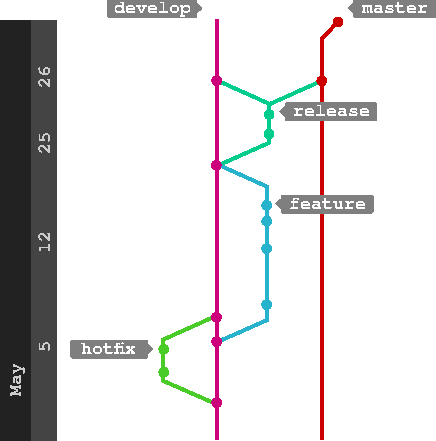
\includegraphics[width=.7\linewidth]{figures/gitflow}  
    \captionof{figure}{Politique de gestion de branches Git adoptée}
    \label{fig:gitflow}
  \end{figure}
  
  Aussi, l'\path{Apploader} a constitué une refonte majeure de l'architecture du logiciel qui a été conceptualisée et développée en équipe. 
  Afin de répartir les tâches que nécessitait son implémentation, nous avons pu expérimenter l'utilisation d'un \gls{Kanban} recensant : 
  \begin{itemize}
   \item les tâches à effectuer, où une tâche dure 2 à 3 jours au maximum 
   \item 
  \end{itemize}

  (planning poker pour l'estimation des tâches en terme de compléxité relative, pemettant de les répartir et les prioriser)
  
\section{Résultats en vue d'un prolongement}  
  \subsection{Un module de SLAM en adéquation avec les attentes du projet}
  
  Nous nous intéressons ici dans un premeir lieu à la fidélité des résultats de SLAM et dans un second temps, à une appréciation de l'ensemble du projet, incluant également les travaux de  M. Chazot et bien sûr la vision de M. Daumand.  
  
  
  Limites d'Hector SLAM 
  
  De plus, la réussite du projet dans sa globalité est attestée par les résultats d'une présentation devant des collaborateurs commerciaux et directeurs de projet qui est intervenue le 13 juin 2017.
  Cette étape a permis de recceuillir des avis extérieurs sur le projet lui-même et d'estimer sa potentielle viabilité commerciale et technique. 
  Ayant été positivement perçu, le système démonstrateur réalisé à été présenté brièvement auprès de Nexter System, enclin à organiser une rencontre à cet effet au mois de septembre. 
  
  
  \subsection{Pourquoi continuer SRT2M}
  
  Ce que l'on a mis en place pour que le projet se prolonge : 
  
  modularité, MAJ, script d 'installation et résolution des dépendances 
  
  potentiel d'apropriation du projet par de tierces personnes facilité : manuel utilisateur en interface web, troubleshooting, documentation automatisée avec Doxygen
  
\section{Retour d'expérience}
  \subsection{Apports et difficultés du projet}
  
  L'adoption des normes de spécification et de conception du logiciel interne a constitué une phase intéressante et complexe à la fois. 
  En effet, la partie Design et Conception de l'IHM, figure \ref{fig:exigences} témoigne d'a prioris au sujet de la conception du logiciel. 
  La DCC003 évoque des ``modules'' --à savoir des exécutables indépendants de l'IHM-- dont l'état devrait apparaitre dans un panneau de contrôle. 
  Or, supposer de la présence de plusieurs exécutables en amont de la conception est un manquement aux préconisations de formalisation du besoin logiciel. 
  Cette partie qui incombe habituellement au futur propriétaire du logiciel a été réalisée en même temps que la conception, d'avantage dans l'optique d'une découverte des normes de spécification que dans celle de réellement 
  s'appuyer sur les documents produits. Le travail s'en est trouvé d'une part simplifié, puisqu'il m'était facile de décrypter un document que j'avais moi-même écrit, et d'autre part complexifié sur le plan du formalisme
  des documents à produire. Cela a principalement engendré des écarts entre les documents de spécification et le code source assez importants, tant et si bien que les parties plus poussées de la documentation en sont 
  rapidement devenues obsolètes. 
  
  Temps d'appropriation du sujet et du domaine qui constitue une découverte, tout autant que les outils utilisés (ROS) ou que les fondements théoriques découverts (SLAM). 
  
  \subsection{\'{E}volution personnelle au sein de la structure}
  
  CDI, sécurité etc... 